\begin{appendices}
\chapter{Touch sensory neurons regain function post injury by establishing cytoplasmic continuity between cut fragments}


\large \textbf{\textit{let-7} miRNA controls CED-7 homotypic adhesion and EFF-1–mediated axonal self-fusion to restore touch sensation following injury}

\small
Atrayee Basu, Shirshendu Dey, Dharmendra Puri, Nilanjana Das Saha, \textbf{Vidur Sabharwal}, Pankajam Thyagarajan, Prerna Srivastava, Sandhya P Koushika, Anindya Ghosh-Roy

Publication date : 21 November 2017
Journal : Proceedings of the National Academy of Sciences
Volume : 114
Issue : 47
doi : \href{https://doi.org/10.1073/pnas.1704372114}{10.1073/pnas.1704372114}

\normalsize
My contributions to the following study include carrying out neuronal injury using a ns-pulsed UV LASER as described in Material and Methods. Following injury, I imaged GFP::RAB-3 labeled vesicles live to assess changes in RAB-3 movement properties in the cell body attached and detached neuronal process post injury. The flux of GFP::RAB-3 decreased in the cell body detached neuronal fragment and only recovered if cytoplasmic continuity was established. Cytoplasmic continuity through a fusion point between the cell body attached and detached fragments led to a rescue of cargo movement in the cell body detached fragment. The close proximity of the two fragments with no cytoplasmic continuity was insufficient to rescue cargo flux in the distal cut fragment. Figures from this article reused under the free use terms stated by PNAS for dissertations.

\section{Introduction}

Neurons may exhibit varying extents of regeneration post injury. This regeneration may be regulated by cell intrinsic and extrinsic factors. There is a growing body of research addressing how regeneration is regulated. As mentioned in the introduction chapter, neuronal regeneration undergoes multiple steps including sensing, signal transmission, transcriptional and translational changes, outgrowth of the neuronal process, sensing the injured fragment and fusion with the distal cut fragment. 

In this study, we decipher the role of a \gls{miRNA} \textit{let-7} in regulating regeneration. \textit{let-7} is a widely expressed hetero-chronic 21 nucleotide long miRNA, which starts expressing around the L4 stage in \textit{C. elegans} \parencite{reinhart2000}. Loss of \textit{let-7} leads to observed larval cell fates in adult animals, while overexpression causes adult cell fates in younger animals \parencite{reinhart2000}. Within \textit{C. elegans} neurons, \textit{let-7} was identified as a positive regulator of regeneration in a reverse genetic screen \parencite{chen2011}. We aimed to address how \textit{let-7} acts as a positive regulator of regeneration.

\section{Results}

\subsection{Cytoplasmic continuity is associated with an increase in GFP::RAB-3 flux within the neuronal process}

To assess how \textit{let-7} coordinates an enhanced recovery of neuronal function post injury, we utilized the behavior of SVP, RAB-3 to assess cargo flux in the neuronal process post injury. Within wild type neurons, 24 hours post-injury, the neuronal process attached to the cell body grows out away from the cell body. If the neuronal process contacts the distal unconnected fragment, it may fuse with either a type 1 fusion (end to end connection), or a type 2 fusion, (end of proximal process may fuse in between the distal fragment) [Fig.~\ref{fig:Atrayeerab}Aa',B]. Alternatively, if the neuron grows out in the wrong direction and does not contact the distal fragment, the distal fragment may undergo degeneration [Fig.~\ref{fig:Atrayeerab}Ab',B].

24 hrs post injury, the GFP::RAB-3 flux within the distal fragment reduces dramatically in both the anterograde and retrograde directions compared to the proximal neuronal process connected to the cell body [Fig.~\ref{fig:Atrayeerab}D,E]. Upon re-connection of the distal with the proximal fragment, the GFP::RAB-3 flux in the distal fragment returns to that observed for the proximal fragment [Fig.~\ref{fig:Atrayeerab}C,E]. In contrast, in a \textit{let-7(lf)} mutant, the GFP::RAB-3 flux remains high even in unfused distal fragments, comparable to that of the proximal fragment [Fig.~\ref{fig:Atrayeerab}F]. Increased GFP::RAB-3 flux may suggest a delayed degeneration response in the distal fragment and may aid in functional recovery. 

	\begin{figure}
	\centering
	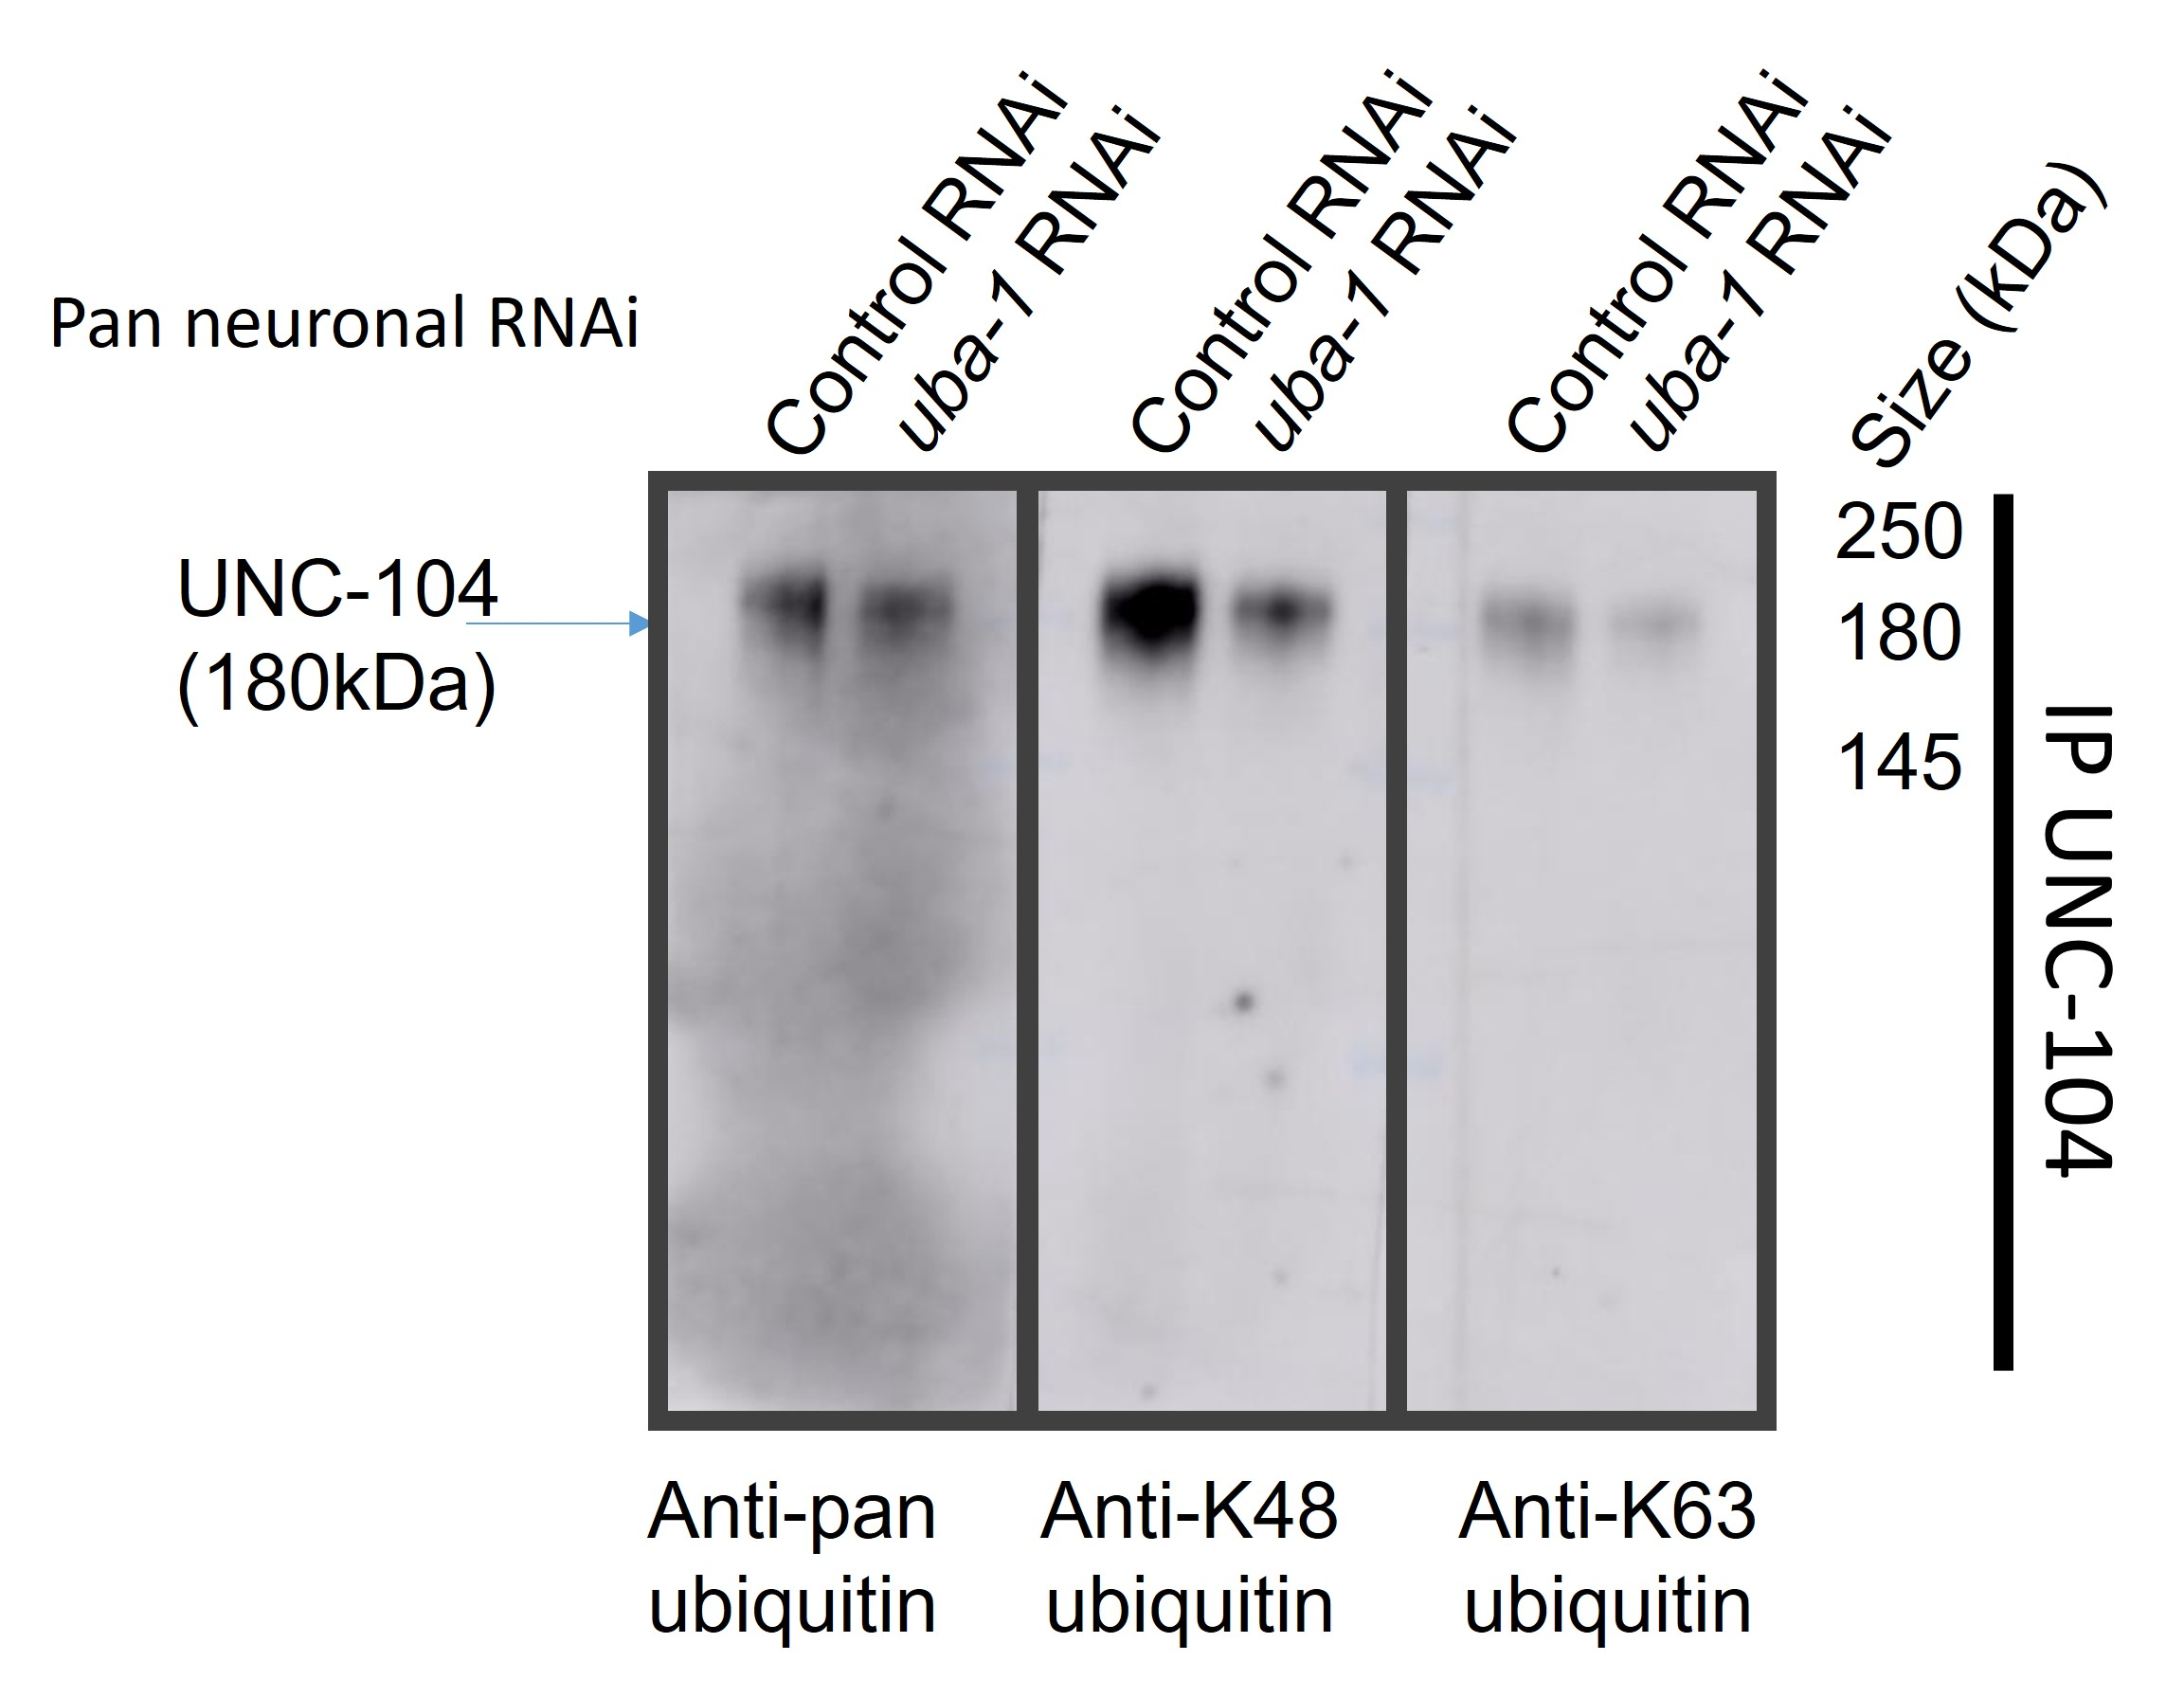
\includegraphics[width=1\linewidth]{figs/example}
	\caption[GFP::RAB-3 flux improves after successful fusion of the cut neuronal processes.]{\textbf{GFP::RAB-3 flux improves after successful fusion of the cut neuronal processes.}} \raggedright \small A) LASER based ablation of the PLM neuron expressing a soluble mCherry along with GFP::RAB-3, shows either a') growth of the proximal process followed by fusion, or b') growth of the proximal process with a failure in fusion with the distal process 24 hours post ablation. B) A schematic showing the traced neuronal processes from A). Representative kymographs of GFP::RAB-3 within the neuronal process with the cell body towards the right either proximal or distal to the cell body post-injury in a C) fusion successful, or D) fusion unsuccessful animal. Yellow arrow indicate anterograde particles, red arrow indicate retrograde particles and white arrow heads indicate stationary GFP::RAB-3 clusters. E) GFP::RAB-3 particle flux in the anterograde (A) or retrograde (R) directions within the proximal (Prox) or distal (Dist) neuronal process in animals with successful or unsuccessful fusion. F) GFP::RAB-3 particle flux in the anterograde (A) or retrograde (R) directions within the proximal (Prox) or distal (Dist) neuronal process in either wild type or \textit{let-7(lf)}. Bar graphs represent averages with the S.E.M. represented as whiskers. One-way ANOVA with Bonferroni test used for all statistical comparisons. ns- non significant, *p$<$0.05 ***p$<$0.001
	\label{fig:Atrayeerab}
\end{figure}

To observe if the fusion of the proximal and distal neuronal processes occurs just to establish cytoplasmic continuity, or if the cytoskeleton themselves are remodeled to create a seamless fusion point, we assessed GFP::RAB-3 movement across the fusion points [Fig.~\ref{fig:Atrayeemontage}]. We observed a smooth movement of GFP::RAB-3 across the fusion point suggesting that the increase in GFP::RAB-3 flux within the distal fragment arises from cargo transport from the proximal fragment.

\begin{figure}[H]
	\begin{minipage}[t]{0.45\textwidth}
%		\mbox{}\\[-\baselineskip]
		\vspace{0pt}
		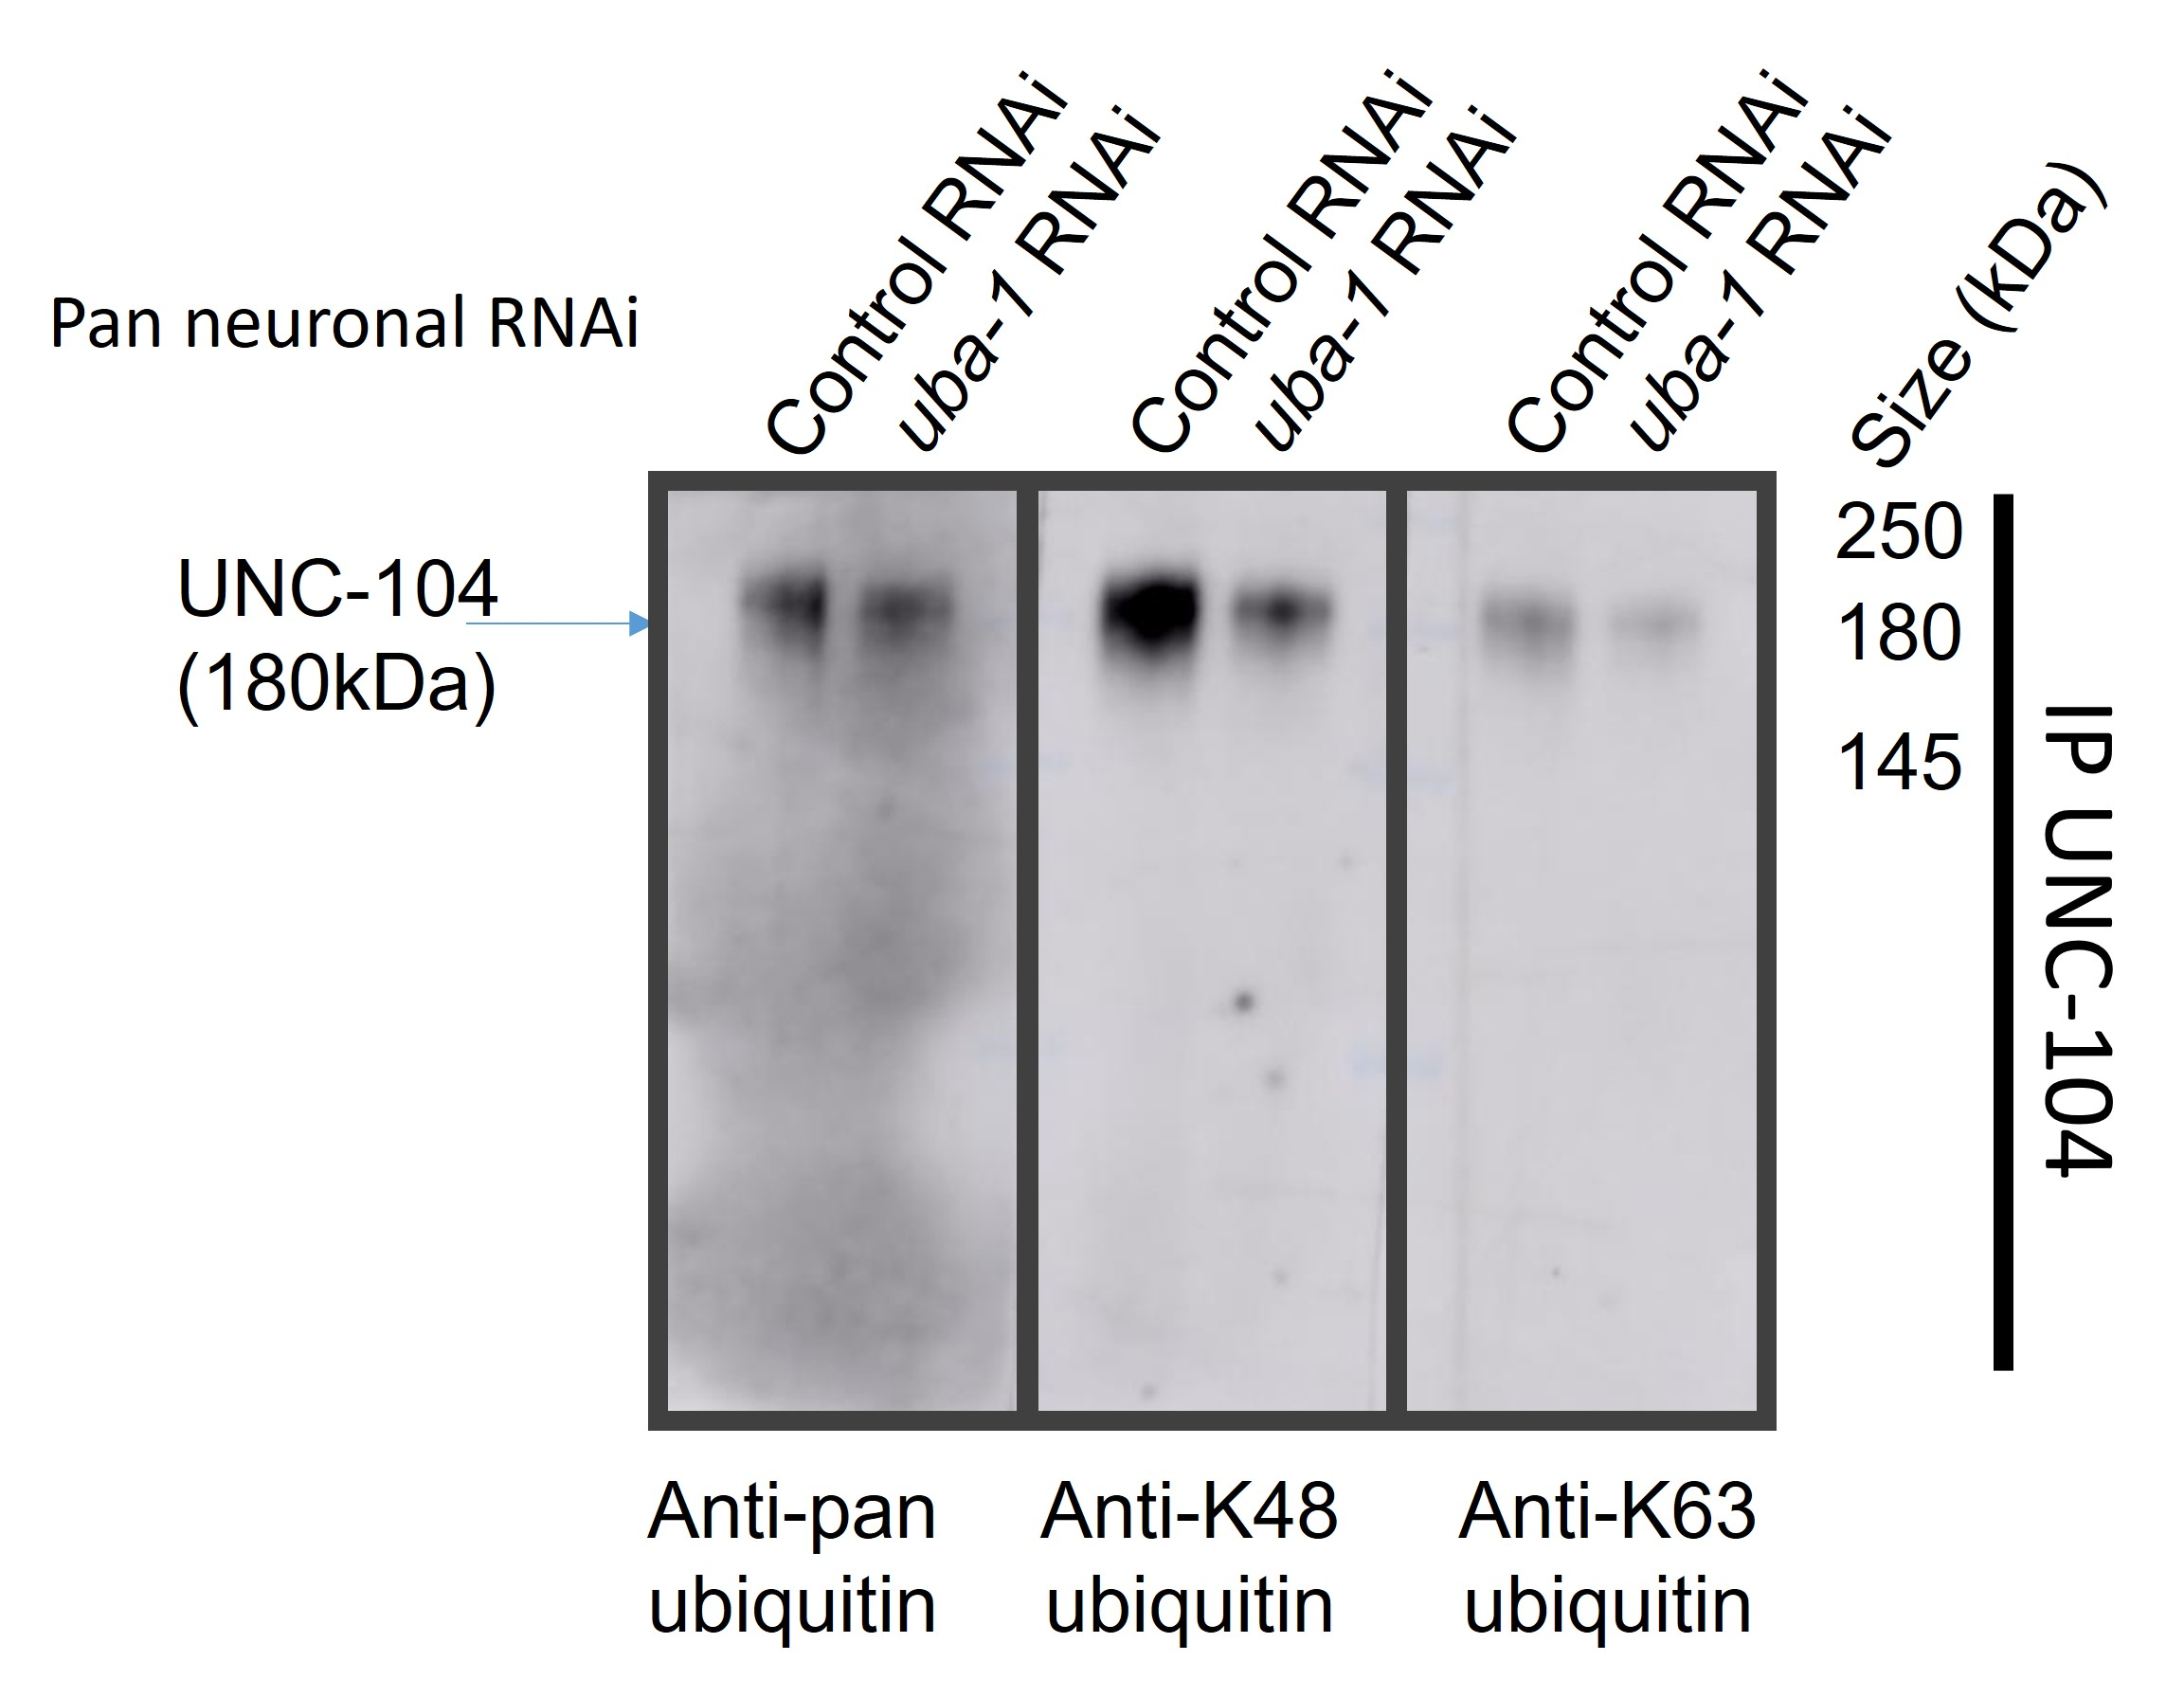
\includegraphics[width=\textwidth]{figs/example}
	\end{minipage}\hfill
	\begin{minipage}[t]{0.5\textwidth}
%		\mbox{}\\[-\baselineskip]
		\vspace{0pt}
		\caption[GFP::RAB-3 cargo movement across a successfully fused neuronal process post injury.]{\textbf{GFP::RAB-3 cargo movement across a successfully fused neuronal process post injury.}} \raggedright \small Montage showing portion of the PLM distal neuronal process expressing GFP::RAB-3 24 hour post injury, with the proximal process fusing in the middle of the distal process. The arrow head labels a single particle that seamlessly crosses the fusion point indicating cytoplasmic continuity between the proximal and distal ends of the neuronal process. Each frame is 250 ms apart. The proximal process, distal process and the fusion point are labeled with arrows. Cell body towards the right. \label{fig:Atrayeemontage}
	\end{minipage}
\end{figure}

	\newcolumntype{L}{>{\RaggedRight\hangafter=1\hangindent=1.5em}X}
	\begin{table}[H]\centering
		\caption{Strain list used in this study}\label{tab:StrainlistA}
		\scriptsize
		\begin{tabularx}{1\textwidth}{@{} l l L l @{}}\toprule
			S. No. &Strain name &Genotype &Reference \\\midrule
			1 &TT2464 &\textit{tbIs222} derived from UV integration of \textit{vdEx263}[(\textit{mec-4p}::\textit{mCherry} (5 ng/μl), \textit{odr-1p}::\textit{dsRed} (30 ng/μl)] &\cite{kirszenblat2013} \\
			2 &NM2689 &\textit{jsIs821} [\textit{mec-7p}::\textit{gfp}::\textit{rab-3}] &\cite{bounoutas2009} \\
			3 & &\textit{let-7(mg279)} &\cite{reinhart2000} \\
			\bottomrule
		\end{tabularx}
	\end{table}
	

\end{appendices}
